\documentclass[11pt,a4paper]{report}

\usepackage{amssymb,amsmath,epsfig,float,subfig,hyperref,multicol}

\usepackage{xcolor}

\definecolor{SCSUred}{HTML}{CD1041}

\hypersetup{colorlinks=true,linkcolor=SCSUred,urlcolor=SCSUred}

\usepackage{enumerate}
\usepackage{tikz}
\usetikzlibrary{arrows}
\usetikzlibrary{patterns}
\usetikzlibrary{decorations}
%%\usetikzlibrary{intersections}
\usetikzlibrary{matrix}
\usetikzlibrary{snakes}
\usetikzlibrary{calc}
\usetikzlibrary{backgrounds}

\definecolor{linecolor}{HTML}{0074C8}
\definecolor{linecolor2}{HTML}{C80200}

\newcommand{\imagebullet}[1]{\includegraphics[width=0.5cm]{#1}}


\pagestyle{empty}
\setlength{\textwidth}{7in}
\setlength{\textheight}{10in}
\setlength{\oddsidemargin}{-25pt}
\setlength{\evensidemargin}{-25pt}
\setlength{\topmargin}{-50pt}

\usepackage[english]{babel}
\usepackage[utf8]{inputenc}
\usepackage{fancyhdr}
 
%%\pagestyle{fancy}
\renewcommand{\headrulewidth}{0pt}
%%\fancyhf{}
%%\rhead{Share\LaTeX}
%%\lhead{Guides and tutorials}
%%\cfoot{OVER}


\newcommand{\DueA}{Thursday, October 17}
\newcommand{\DueB}{Monday, October 21}
\newcommand{\DueC}{Monday, October 28}

\begin{document}


\begin{figure}[ht]
\begin{flushright}
	\includegraphics[width=2.0in]{U_PriHorz_WhtLtBG.jpg}
	\end{flushright}
\end{figure}

\vspace{-12mm}

\begin{flushleft}
\Large\bf \href{https://activecalculus.org/single/sec-2-8-LHR.html}{2.8 - Using Derivatives to Evaluate Limits}\rm
%%Daily Preparation - \DueA \rm
\end{flushleft}


\vspace{8pt}

\noindent {\Large\bf{Overview}} \\
As we complete Chapter 2 and move on to Chapter 3, the theme of our work will focus on how we can apply the meaning of the derivative to solve important problems. Interestingly, although we use limits to define the derivative itself, it turns out that the derivative can be a useful tool in evaluating challenging limits of a certain type.\\

\noindent
The topics discussed in this section are: Indeterminate forms of type ``0/0". Local linearization and L'H\^{o}pital's Rule. Infinite limits and limits at infinity. Asymptotes. Indeterminate forms of type ``$\infty/\infty$". Indeterminate products of the form `$0 \cdot \infty$". Indeterminate powers of the form ``$\infty^0$", ``$1^{\infty}$", ``$0^0$".






\vspace{16pt}

%%\pagebreak

\noindent {\Large\bf{To prepare for class}} \\
Complete all actions listed below.  Respond to the questions highlighted with {\color{SCSUred}{\boxed{Submit}}}.  %% by the start of class on {\bf{\DueA}}.  A single .pdf should be uploaded to D2L Brightspace.
\begin{itemize} \itemsep -2pt % Reduce space between items

\item {\bf{Read}} motivating questions and the introduction to \href{https://activecalculus.org/single/sec-2-8-LHR.html}{section 2.8} (up until Preview Activity 2.8.1).

\item[\imagebullet{CopilotLogo.jpg}] Ask {\bf{Copilot}} ``What is meant by an indeterminant form of a limit?"

\item[{\color{SCSUred} \boxed{Submit}}]  {\bf{Do}} \href{https://activecalculus.org/single/sec-2-8-LHR.html#tAL}{Preview Activity 2.8.1}.
\begin{itemize}\itemsep -2pt % Reduce space between items
\item (Optional) {\bf{Watch}} video \href{https://www.youtube.com/watch?v=-FA6V_tmPuA}{solution to Preview Activity 2.8.1}.
\end{itemize}

\item {\bf{Read}} \href{https://activecalculus.org/single/sec-2-8-LHR.html#SpQ}{section 2.8.1}.

\item[{\color{SCSUred} \boxed{Submit}}] {\bf{Do}} the following construction in \href{https://www.geogebra.org/classic}{GeoGebra}.  Note how the red graph of the quotient $h(x)$ suggests that $\displaystyle \lim_{x\rightarrow 1} \frac{x^5+x-2}{x^2-1} = 3$.  The value of $b$ is what is computed via L'H\^{o}pital's rule.  
\begin{figure}[H]
\begin{center}
	\includegraphics[width=4.75in]{LHopitalGeoGebra1.jpg}
\end{center}
\end{figure}
Repeat this construction to analyze the limit found in \href{https://activecalculus.org/single/sec-2-8-LHR.html#vpu}{Activity 2.8.2(a)}.  That is, use $f(x) = \ln(1+x)$, $g(x) = x$, and investigate the limit of $f(x)/g(x)$ as $x \rightarrow 0$.  Submit screenshots as needed.

\item[{\color{SCSUred} \boxed{Submit}}]  {\bf{Do}} form a table of values using a spreadsheet ({\it{Excel}} or {\it{Google Sheets}}) to form a hypothesis regarding the value of $\displaystyle \lim_{x \rightarrow 0} \frac{e^{2x}-1}{x}$.  Values of $x$ that are both negative and positive near zero should be used.  Then, repeat the {\it{GeoGebra}} exploration above to see if the same value for the limit emerges.  [Yes, you should get 2.]  Sample output is shown below.  Submit screenshots as needed.  
\begin{figure}[H]
\begin{center}
	\includegraphics[width=3.5in]{LHopitalExcel1.jpg}
\end{center}
\end{figure}


\item {\bf{Do}} the following problem.
\begin{enumerate}
\item We attempt to evaluate the value of $\displaystyle \lim_{x \rightarrow 0} \frac{e^{2x}-1}{x}$.  Define $f(x) = e^{2x}-1$ (the numerator) and define $g(x) = x$ (the denominator).  Then $\displaystyle \lim_{x \rightarrow 0} \frac{e^{2x}-1}{x} = \lim_{x \rightarrow 0} \frac{f(x)}{g(x)}.$
\begin{enumerate}
\item Does  $\displaystyle \lim_{x \rightarrow 0} \frac{f(x)}{g(x)} = \frac{f(0)}{g(0)}$?  Why or why not?  
%%\vspace{20mm}
\item Find the linear approximation $L(x)$ to $f(x)$ at $a=0$.  
%%\vspace{20mm}
\item Find the linear approximation $M(x)$ to $g(x)$ at $a=0$.  
%%\vspace{20mm}
\item Compute $\displaystyle \lim_{x \rightarrow 0} \frac{L(x)}{M(x)}$.  How is this related to $\displaystyle \frac{f'(0)}{g'(0)}$? 
%%\vspace{25mm} 
\item For $x$ near 0, $$\frac{f(x)}{g(x)} = \frac{e^{2x}-1}{x} \approx \frac{2x}{x} = \frac{L(x)}{M(x)} = \frac{f'(0)}{g'(0)}.$$  As $x \rightarrow 0$, the approximation becomes better.  This tells us $\displaystyle \lim_{x \rightarrow 0} \frac{e^{2x}-1}{x} = {\underline{\hspace{30mm}}}$.
%%\vspace{15mm}
\end{enumerate}  


\end{enumerate}

\item {\bf{Watch}} video \href{https://www.youtube.com/watch?v=KXGhzie3b8s&feature=emb_title}{Quick Review - L'Hopital's Rule (3:27)}.   

\item {\bf{Watch}} video \href{https://www.youtube.com/watch?v=flM7qVLdezY&feature=emb_title}{Using L'Hopital's Rule with Zero (7:26)}. 



%%\item {\bf{Do}} \href{https://activecalculus.org/single/sec-2-8-LHR.html#vpu}{Activity 2.8.2}.

%%\item {\bf{Do}} \href{https://activecalculus.org/single/sec-2-8-LHR.html#Fta}{Activity 2.8.3}.  

\item {\bf{Do}} \href{https://activecalculus.org/single/sec-2-8-LHR.html#qtK}{Exercises 1-2 in section 2.8.4}. 







\end{itemize}





\vspace{16pt}

\noindent {\Large\bf{After class}}\\
Solidifying the concepts discussed in class through practice is necessary to build your skills. 

%%\noindent {\large\bf{After \DueA}}
\begin{itemize}\itemsep -2pt % Reduce space between items
\item {\bf{Read}} \href{https://activecalculus.org/single/sec-2-8-LHR.html#ywZ}{section 2.8.2}.
\item {\bf{Watch}} video \href{https://www.youtube.com/watch?v=wXXej6AmEKQ&feature=emb_title}{Using L'Hopital's Rule with Infinity (8:45)}.  

\item[\imagebullet{CopilotLogo.jpg}] Ask {\bf{Copilot}} ``How can I use L'Hopital's rule to compute the value of a limit that is in the form 0$\wedge$0?"

\item {\bf{Read}} \href{https://activecalculus.org/single/sec-2-8-LHR.html#eEi}{section 2.8.3 (summary)}.



\item {\bf{Do}} \href{https://activecalculus.org/single/sec-2-8-LHR.html#rkI}{Exercises 3-4 in section 2.8.4}.





 
\item {\bf{Do}} these problems.
\begin{enumerate}
\setcounter{enumi}{1}
\item Compute each of the following limits exactly.  
\begin{enumerate}
\item $\displaystyle \lim_{x \rightarrow 0} \frac{\sin x}{x}$
%%\vspace{25mm}
\item $\displaystyle \lim_{x \rightarrow 0} \frac{x}{e^x}$
%%\vspace{25mm}
\item $\displaystyle \lim_{t \rightarrow 0}\frac{e^t - 1 - t}{t^2}$
%%\vspace{25mm}
\end{enumerate} 



\item Find the sign of $\displaystyle \lim_{x \rightarrow a} \frac{f(x)}{g(x)}$ from the figure.  \\ Assume $f''(a) \neq 0$ and $g''(a) \neq 0$.  

\vspace{-40mm}
   \begin{figure}[H]
\flushright
{
  \begin{tikzpicture}[thick,scale=1.1] [domain=-3:3]
%%\draw[step=1cm,color=gray!50,dotted] (0,-3) grid (5,3);
   \draw [black!80,line width=0.3pt,-latex] (0,0) -- (3,0) node [below] at (2.75,0) {$x$};
   \draw [black!80,line width=0.3pt,-latex] (0,0) -- (-0.5,0);
   \draw [black!80,line width=0.3pt,-latex] (0,0) -- (0,3) node [right] at (0,2.75) {$y$};
   \draw [black!80,line width=0.3pt,-latex] (0,0) -- (0,-1);
\draw[color=blue, line width=1pt,domain=0:1]   plot (\x,{(\x-1)^2}) node [right] at (0.25,1) {$f(x)$};
\draw[color=blue, line width=1pt,domain=1:2]   plot (\x,{(\x-1)^3});
\draw[color=blue, line width=1pt,domain=2:2.5]   plot (\x,{-(\x-2)^3+1});
\draw[color=red, line width=1pt,domain=1:2]   plot (\x,{-(\x-1)^2}) node [right] at (0.25,-1) {$g(x)$};
\draw[color=red, line width=1pt,domain=0:1]   plot (\x,{0.5*(\x-1)^3});
%%  node[above] at (2,1) {$f(3,y)$};
\foreach \x/\xtext in { 1/a}
    \draw[shift={(\x,0)}] (0pt,3pt) -- (0pt,-3pt) node[below] {$\xtext$};
%%\foreach \y/\ytext in {-3/-3, -2/-2, -1/-1, 1/1, 2/2, 3/3}
    %%\draw[shift={(0,\y)}] (-2pt,0pt) -- (2pt,0pt) node[left] {$\ytext$};
\end{tikzpicture}}  
\end{figure}



\end{enumerate}

%%\item {\bf{Do}} Activity 2.8.4.   

%%\end{itemize}

%%\pagebreak

%%\vspace{-10mm}
%%\noindent {\large\bf{After \DueB}}
%%\begin{itemize}\itemsep -2pt % Reduce space between items 
 



 

\item {\bf{Do}} \href{https://activecalculus.org/single/sec-2-8-LHR.html#Dza}{Exercises 5-8 from section 2.8.4}.

\item {\bf{Start working}} on the \href{https://www.myopenmath.com/index.php}{MOMwork} (MyOpenMath) assignment for this section.  %%This will be due on \DueC. 

\end{itemize}

%%\pagebreak

\vspace{16pt}

\noindent {\Huge\bf{Extra Prep}}

\vspace{16pt}

\noindent {\Large\bf{Basic learning objectives}}\\
These are the tasks you should be able to perform with reasonable
fluency when you arrive at our next class meeting. Important new
vocabulary words are indicated {\it{in italics}}.  Check each box when you feel confident you have a firm grasp on that objective.  

\begin{itemize} \itemsep -2pt % Reduce space between items
\renewcommand{\labelitemi}{\scriptsize$\square$}
\item State what it means to say that a limit has an indeterminate form and how such forms arise in the limit definition of the derivative.
\item State L'H\^{o}pital's Rule.

\item Explain how L'H\^{o}pital's Rule is used to calculate limits having an indeterminate form.

\item Explain what the expression $\displaystyle \lim_{x \rightarrow \infty} f(x) = L$ means in plain English.

\item State the ``$\infty$'' version of L'H\^{o}pital's Rule.
\end{itemize}

\vspace{16pt}

\noindent {\Large\bf{Advanced learning objectives}}\\
In addition to mastering the basic objectives, here are the tasks you should be able to perform after class, with practice:
\begin{itemize} \itemsep -2pt % Reduce space between items
\item Understand the development of L'H\^{o}pital's Rule and how it relies upon the tangent line approximation of two functions.

\item Use L'H\^{o}pital's Rule to calculate limits that have an indeterminate form ``0/0".

\item Use L'H\^{o}pital's Rule to calculate limits that have an indeterminate form ``$\infty/\infty$".

\item Use limits to identify locate horizontal and vertical asymptotes.

\item Find limits involving indeterminate products (``$0\cdot \infty$"): rewrite the limit in such a way that L'H\^{o}pital's Rule can be used.

\item Find limits involving indeterminate powers (``$\infty^0$", "$1^\infty$", "$0^0$"): use the identity $u=e^{\ln u}$ to rewrite the expression and find the limit of the exponent (you may get an indeterminate power and L'H\^{o}pital's Rule might be required at this point).

\item Realize which forms of limits are not indeterminate, i.e. which always result in a clear answer (e.g. ``$0^{\infty}$"=0, ``$*/\infty$"=0, ``$*/0^+$"=$\infty$)
\end{itemize}

\vspace{16pt}

\noindent {\Large\bf{Need More Help?}}

\begin{itemize}\itemsep -2pt % Reduce space between items
\item {\bf{Watch}} video \href{https://www.youtube.com/watch?v=IZNU_ZQuPQM&feature=emb_title}{L'Hopital's Rule - A Graphical Approach (10:52)}.  


\item {\bf{Watch}} video \href{https://www.youtube.com/watch?v=OygUfugpQ48&feature=youtu.be}{Student Problem Solving - L'Hopital's Rule (3:20)}.

\item {\bf{Watch}} video \href{https://www.youtube.com/watch?v=SkWMqPeSC7I&feature=youtu.be}{Limit of Quotients (6:56)}.

\item {\bf{Watch}} video \href{https://www.youtube.com/watch?v=fZXVSwYtctU&feature=emb_title}{Indeterminant Products (9:07)}.  

\item {\bf{Watch}} video \href{https://www.youtube.com/watch?v=tbgH97QAntw&feature=emb_title}{Horizontal Asymptotes and Limits at Infinity (6:16)}.  

\item {\bf{Watch}} video \href{https://www.youtube.com/watch?v=zONlxdjhrUs&feature=emb_title}{L'Hopital's Rule and Limits of the Form 0 x Infinity (9:09)}.

\item {\bf{Do}} these problems.
\begin{enumerate}
\setcounter{enumi}{3}
\item Evaluate $\displaystyle \lim_{x \rightarrow 1} \left( \frac{x}{x-1} - \frac{1}{\ln x} \right)$.  

\pagebreak

\item Use the graphs of $f$ and $g$ and their tangent \\
lines at $(2,0)$ to find $\displaystyle \lim_{x \rightarrow 2} \frac{f(x)}{g(x)}$.  

\vspace{-15mm}
 \begin{figure}[H]
\flushright
{
  \begin{tikzpicture}[thick,scale=1] 
\draw[step=1cm,color=gray!50] (-1,-2) grid (5,5);
   \draw [black!80,line width=0.3pt,-latex] (0,0) -- (5.25,0)
   node [below] at (4.75,0) {$x$};
   \draw [black!80,line width=0.3pt,-latex] (0,0) -- (-1.5,0);
   \draw [black!80,line width=0.3pt,-latex] (0,0) -- (0,5.25)
   node [left] at (0,4.75) {$y$};
   \draw [black!80,line width=0.3pt,-latex] (0,0) -- (0,-2.5);
      \draw [black] node [below] at (2.5,0) {$(2,0)$};
\draw[color=red, line width=1.5pt,dotted,domain=-0.5:4.5]   plot (\x,{0.8*(\x-2)}) node [right] at (4.5,1.75) {$y=\frac{4}{5}(x-2)$};
\draw[color=red, line width=1.5pt,domain=1.05:4.75]   plot (\x,{0.8*ln(\x-1)}) node [right] at (4.5,0.5) {$f$};
\fill [black] (2,0) circle (3pt);

\draw[color=linecolor, line width=1.5pt,dotted,domain=1:4.5]   plot (\x,{1.8*(\x-2)}) node [right] at (4.5,4) {$y=1.8(x-2)$};
\draw[color=linecolor, line width=1.5pt,domain=1.2:4.75]   plot (\x,{1.8*ln(\x-1)}) node [right] at (4.75,2.5) {$g$};

\end{tikzpicture}}  
\end{figure}

\item Calculate $\displaystyle \lim_{x \rightarrow \infty} \left( 1 + \frac{1}{x} \right)^x$.  {\it{Hint:}} Note that this limit has the form $1^{\infty}$.  So write $$y=\left( 1 + \frac{1}{x} \right)^x$$ and find the limit of $\ln y$. 

\item Put the following limits in a form that can be evaluated using L'H\^opital's rule.
\begin{enumerate}
\item $\displaystyle \lim_{x \rightarrow \infty} x^{1/x}$  \ \ {\it{Hint:}} Use a logarithm.
%%\vspace{45mm}
\item $\displaystyle \lim_{x \rightarrow 0^+} x^x$  \ \ {\it{Hint:}} Use a logarithm.
%%\vspace{45mm}
\item $\displaystyle \lim_{x \rightarrow 0} \frac{1}{x} - \frac{1}{\sin x}$
%%\vspace{35mm}
\end{enumerate}

\item Compute each of the following limits exactly.  
\begin{enumerate}
\item $\displaystyle \lim_{x \rightarrow \infty} \frac{\ln x}{x}$
%%\vspace{15mm}
\item $\displaystyle \lim_{x \rightarrow \infty} \frac{\ln (\ln x)}{\sqrt{x}}$
%%\vspace{20mm}
\end{enumerate} 

\item Calculate $\displaystyle \lim_{x \rightarrow \infty} xe^{-x}$.  {\it{Hint:}} Note that this limit has the form $\infty \cdot 0$.  Rewrite $\displaystyle xe^{-x} = \frac{x}{e^x}$ so that the limit takes the form $\displaystyle \frac{\infty}{\infty}$.



\end{enumerate}

\item {\bf{Watch}} video \href{https://www.youtube.com/watch?v=SjCDSQJln3g&list=PLJtEcQL1-E8V9Fs1E1-KY9nyL9y2JHh8-&index=21}{Indeterminant Forms (6:47)}. 

\item {\bf{Watch}} video \href{https://www.youtube.com/watch?v=LqdKmnh3h-k&list=PLJtEcQL1-E8V9Fs1E1-KY9nyL9y2JHh8-&index=20}{More Indeterminant Forms (6:01)}.
\end{itemize}

 \vspace{16pt}

\noindent {\Large\bf{Selected Answers}}
\begin{enumerate}
\setcounter{enumi}{0}

\item 
\begin{enumerate}
\item $f(0)=0$ and $g(0)=0$ so clearly not.
\item $f'(0)=2$ means that $L(x) = 2x$.
\item $M(x) = x$
\item 2; it is the same.
\item 2
\end{enumerate}

\item 
\begin{enumerate}
\item 1
\item 1
\item $\displaystyle \frac{1}{2}$
\end{enumerate}

\item Negative.  

\item $\displaystyle \frac{1}{2}$

\item $\displaystyle \frac{4}{9}$

\item $e$

\item 
\begin{enumerate}
\item 1
\item 1
\item 0
\end{enumerate}

\item 
\begin{enumerate}
\item 0
\item 0
\end{enumerate}

\item 0


\end{enumerate}

 

\end{document}

